\documentclass[11pt,]{article}
\usepackage[left=1in,top=1in,right=1in,bottom=1in]{geometry}
\newcommand*{\authorfont}{\fontfamily{phv}\selectfont}
\usepackage[]{mathpazo}


  \usepackage[T1]{fontenc}
  \usepackage[utf8]{inputenc}



\usepackage{abstract}
\renewcommand{\abstractname}{}    % clear the title
\renewcommand{\absnamepos}{empty} % originally center

\renewenvironment{abstract}
 {{%
    \setlength{\leftmargin}{0mm}
    \setlength{\rightmargin}{\leftmargin}%
  }%
  \relax}
 {\endlist}

\makeatletter
\def\@maketitle{%
  \newpage
%  \null
%  \vskip 2em%
%  \begin{center}%
  \let \footnote \thanks
    {\fontsize{18}{20}\selectfont\raggedright  \setlength{\parindent}{0pt} \@title \par}%
}
%\fi
\makeatother




\setcounter{secnumdepth}{3}


\usepackage{graphicx,grffile}
\makeatletter
\def\maxwidth{\ifdim\Gin@nat@width>\linewidth\linewidth\else\Gin@nat@width\fi}
\def\maxheight{\ifdim\Gin@nat@height>\textheight\textheight\else\Gin@nat@height\fi}
\makeatother
% Scale images if necessary, so that they will not overflow the page
% margins by default, and it is still possible to overwrite the defaults
% using explicit options in \includegraphics[width, height, ...]{}
\setkeys{Gin}{width=\maxwidth,height=\maxheight,keepaspectratio}

\title{\textbar{}Preferencia de nidos de hormigas en el campus universitario
UASD \textbar{} \textbar{}  }



\author{\Large Enrique A. García Vargas\vspace{0.05in} \newline\normalsize\emph{Estudiante, Universidad Autónoma de Santo Domingo (UASD)}  }


\date{}

\usepackage{titlesec}

\titleformat*{\section}{\normalsize\bfseries}
\titleformat*{\subsection}{\normalsize\itshape}
\titleformat*{\subsubsection}{\normalsize\itshape}
\titleformat*{\paragraph}{\normalsize\itshape}
\titleformat*{\subparagraph}{\normalsize\itshape}

\titlespacing{\section}
{0pt}{36pt}{0pt}
\titlespacing{\subsection}
{0pt}{36pt}{0pt}
\titlespacing{\subsubsection}
{0pt}{36pt}{0pt}





\newtheorem{hypothesis}{Hypothesis}
\usepackage{setspace}

\makeatletter
\@ifpackageloaded{hyperref}{}{%
\ifxetex
  \PassOptionsToPackage{hyphens}{url}\usepackage[setpagesize=false, % page size defined by xetex
              unicode=false, % unicode breaks when used with xetex
              xetex]{hyperref}
\else
  \PassOptionsToPackage{hyphens}{url}\usepackage[unicode=true]{hyperref}
\fi
}

\@ifpackageloaded{color}{
    \PassOptionsToPackage{usenames,dvipsnames}{color}
}{%
    \usepackage[usenames,dvipsnames]{color}
}
\makeatother
\hypersetup{breaklinks=true,
            bookmarks=true,
            pdfauthor={Enrique A. García Vargas (Estudiante, Universidad Autónoma de Santo Domingo (UASD))},
             pdfkeywords = {Hormigas, Ambiente urbano},  
            pdftitle={\textbar{}Preferencia de nidos de hormigas en el campus universitario
UASD \textbar{} \textbar{}},
            colorlinks=true,
            citecolor=blue,
            urlcolor=blue,
            linkcolor=magenta,
            pdfborder={0 0 0}}
\urlstyle{same}  % don't use monospace font for urls

% set default figure placement to htbp
\makeatletter
\def\fps@figure{htbp}
\makeatother

\usepackage{pdflscape} \newcommand{\blandscape}{\begin{landscape}}
\newcommand{\elandscape}{\end{landscape}}


% add tightlist ----------
\providecommand{\tightlist}{%
\setlength{\itemsep}{0pt}\setlength{\parskip}{0pt}}

\begin{document}
	
% \pagenumbering{arabic}% resets `page` counter to 1 
%
% \maketitle

{% \usefont{T1}{pnc}{m}{n}
\setlength{\parindent}{0pt}
\thispagestyle{plain}
{\fontsize{18}{20}\selectfont\raggedright 
\maketitle  % title \par  

}

{
   \vskip 13.5pt\relax \normalsize\fontsize{11}{12} 
\textbf{\authorfont Enrique A. García Vargas} \hskip 15pt \emph{\small Estudiante, Universidad Autónoma de Santo Domingo (UASD)}   

}

}








\begin{abstract}

    \hbox{\vrule height .2pt width 39.14pc}

    \vskip 8.5pt % \small 

\noindent El objetivo de este trabajo consistió en hacer un análisis de la
composición de las poblaciones de hormigas en la Universidad Autónoma de
Santo Domingo e identificar cuales factores pueden afectar la
preferencia de nidos y cual especie es la mejor adaptada en este
ambiente urbano.


\vskip 8.5pt \noindent \emph{Keywords}: Hormigas, Ambiente urbano \par

    \hbox{\vrule height .2pt width 39.14pc}



\end{abstract}


\vskip 6.5pt


\noindent  \section{Introducción}\label{introducciuxf3n}

La urbanización implica la alteración de un ecosistema para beneficio
humano, esto trae como consecuencia la perdida de especies nativas y a
la disminución de la bio diversidad (McKinney, 2002). Sin embargo esto
también crea heterogeneda en el habitat lo que beneficia, principalmente
a las especies mejores adaptados a este tipo de ecosistemas. Mientras
que animales vertebrados y plantas requieren de zonas grandes, los
parches pequeños son suficientes para pequeños organismos.(McKinney,
2008)

En la universidad Autónoma de santo domingo se pueden identificar 4
tipos diferentes de habitats edificación erguida, construido (bordes
edificios, acerado, bancos, postes\ldots{}) suelo, no edificado ni
cubierto y dosel.

Los artrópodos son ideales para estudiar los efectos de la urbanización
gracias a su corto ciclo de vida, su facilidad de muestreo, a su
importancia en la cadena trófica y sirven como bioindicadores
importantes para los cambios ecológicos. (McIntyre, 2000)

Las hormigas son una buena opción a la hora de estudiar las de zonas
urbanas gracias a su facilidad de adaptación, su abundancia y facilidad
para recolección ( Holway, Lach, Suarez, Tsutsui, \& Case (2002)).

Las especies invasoras son uno de los factores que afectan a las
especies nativas, estos tienden a prosperar en habitats urbanos y a
desplazar especies locales (Agosti, Majer, Alonso, \& Schultz, 2000).

En la República Dominicana no existen muchos articulo sobre la
composición de hormigas en ambientes urbanos, por lo que este trabajo
pretende el estudio de especie en zonas urbanas y como estos son
afectados por el mismo.

\section{Metodología}\label{metodologuxeda}

Se dividió el área de la Universidad Autónoma de Santo Domingo en 189
parcelas y se seleccionaron 13 parcelas (6 próximas y 7 alejadas de
sitios a comida) de 50 metros cuadrados.
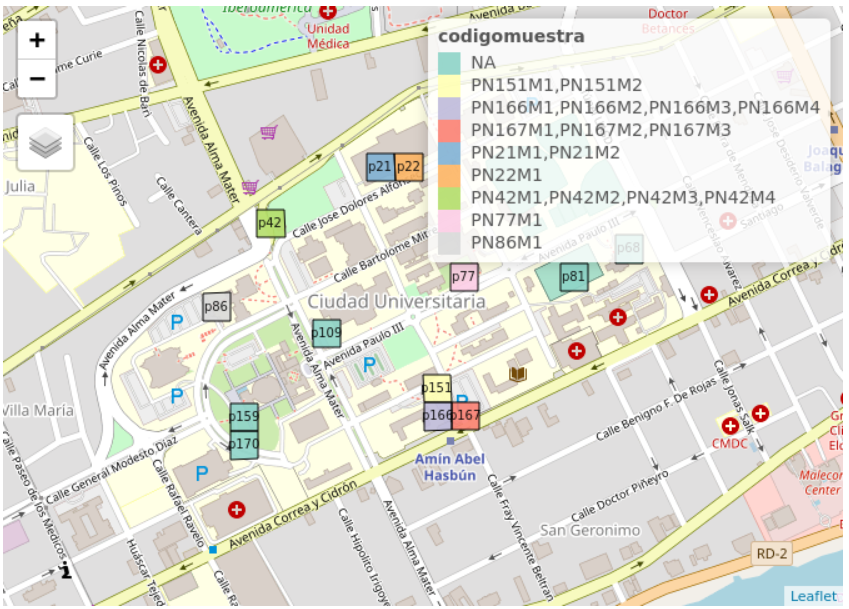
\includegraphics{img/area de estudio y parcelas.png} Se recorrieron los
transectos seleccionadas y se recolectaban muestras de hormigas de los
hormigueros observados, aparte se anotaba información pertinente. Esto
incluyen cercanía con caminos, tanques de basura y agua estancada, Así
como las coordenadas de los nidos y el tipo de cubierta predominante de
la parcela.

Para la recolección se utilizó un pincel de hebras suaves y las hormigas
se almacenaban en tubos plásticos con alcohol etílico al 80\%.

Se observabaron las hormigas con una lupa de mesa y la identificación de
las hormigas se realizo usando la paguina Antwiki.org.

Se utilizó Rstudio para la realización de las tablas y el manuscrito. \#
Resultados

Se observaron 13 nidos totales con una riqueza de 3 especies en los
trancemos analizados.(figura 1)

\begin{figure}
\centering
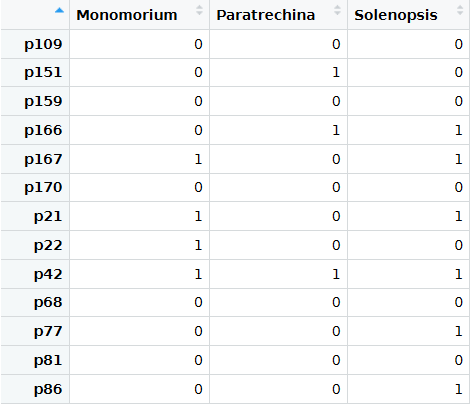
\includegraphics{img/presencia de especies.png}
\caption{presencia de especies por parcela}
\end{figure}

En los trancemos próximas a sitios de comida se promediaron 1.8 especies
mientras que en las parcelas alejadas a sitios de comida el promedio de
especies fue de 0.3.

Las zonas de suelo no edificados ni cubiertos y edificaciones se
encontraron el mismo numero de muestras con los trancemos en suelo no
edificados teniendo la mayor diversidad de especies.La mayoría de nidos
fueron encontrados a una distancia de 1 a 5 metros de basureros y en
general no se encontraron cerca de zonas de agua. (figura 2)

\begin{figure}
\centering
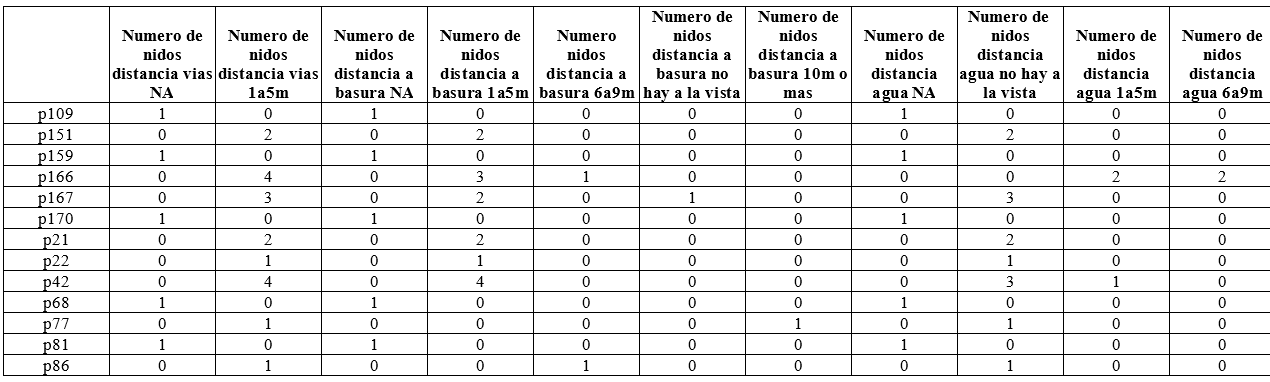
\includegraphics{img/distancias.png}
\caption{Se puede observar como la mayoria de nidos se encuentran con
proximidad a basura mientras que los demas factores no parecen ser
significantes.}
\end{figure}

Solenopsis tenia preferencia de suelos herbaceos no cubiertos ni
construidos, monomorium tenia preferencia a zonas con edificación
erguidas y paratrechina a zonas tipo borde de edificios. (figura 3)

\begin{figure}
\centering
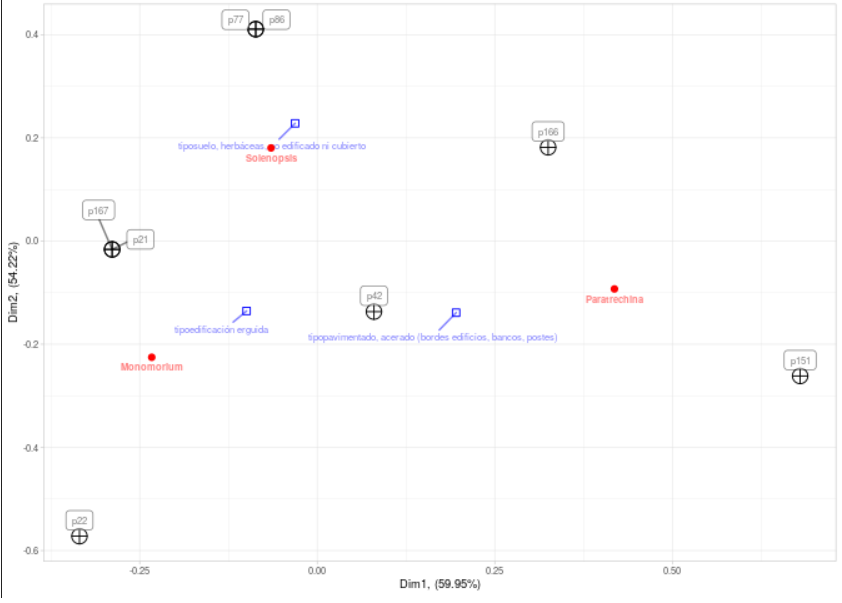
\includegraphics{img/preferencias de hormigas.png}
\caption{En este biplot podemos observar como cada especie en que tipo
de suelo suele encontrarce cada tipo de hormiga}
\end{figure}

\section{Discusión}\label{discusiuxf3n}

Los resultados parecen indican que La mayoría de las especies
encontradas son invasoras, siendo el genero más común solenopsis lo que
puede indicar que están mejor adaptadas para las zonas alteradas, los
datos recolectados parecen indicar que los vertederos y sitios de
comidas son factores que afectan la preferencia de nidos de las hormigas
mientras que proximidad al agua no parece ser un factor determinante.

Si se realizan más muestreos es probable que el numero de especies
aumenten.

\section{Agradecimientos}\label{agradecimientos}

Agracimiento al profesor Jose Martines.

\section*{Referencias}\label{referencias}
\addcontentsline{toc}{section}{Referencias}

\hypertarget{refs}{}
\hypertarget{ref-agosti2000ants}{}
Agosti, D., Majer, J., Alonso, L. E., \& Schultz, T. (2000). \emph{Ants:
Standard methods for measuring and monitoring biodiversity}. Smithsonian
Institution Press.

\hypertarget{ref-holway2002causes}{}
Holway, D. A., Lach, L., Suarez, A. V., Tsutsui, N. D., \& Case, T. J.
(2002). The causes and consequences of ant invasions. \emph{Annual
Review of Ecology and Systematics}, \emph{33}(1), 181--233.

\hypertarget{ref-mcintyre2000ecology}{}
McIntyre, N. E. (2000). Ecology of urban arthropods: A review and a call
to action. \emph{Annals of the Entomological Society of America},
\emph{93}(4), 825--835.

\hypertarget{ref-mckinney2002urbanization}{}
McKinney, M. L. (2002). Urbanization, biodiversity, and conservationthe
impacts of urbanization on native species are poorly studied, but
educating a highly urbanized human population about these impacts can
greatly improve species conservation in all ecosystems.
\emph{Bioscience}, \emph{52}(10), 883--890.

\hypertarget{ref-mckinney2008effects}{}
McKinney, M. L. (2008). Effects of urbanization on species richness: A
review of plants and animals. \emph{Urban Ecosystems}, \emph{11}(2),
161--176.




\newpage
\singlespacing 
\end{document}
